\documentclass[xcolor=table]{beamer}

\usetheme[secheader,compress]{Madrid} %Primary theme

\usepackage{verbatim}
\usepackage{graphicx}

%% UTM Colors
\definecolor{UTMblue}{rgb}{0.043137, 0.137254, 0.254901}
\definecolor{UTMorange}{rgb}{1.0, 0.509803, 0}

\setbeamercolor{palette primary}{bg=UTMblue,fg=white}
\setbeamercolor{palette secondary}{bg=UTMblue,fg=white}
\setbeamercolor{palette tertiary}{bg=UTMblue,fg=white}
\setbeamercolor{palette quaternary}{bg=UTMblue,fg=white}
\setbeamercolor{structure}{fg=UTMblue} % itemize, enumerate, etc
\setbeamercolor{section in toc}{fg=UTMblue} % TOC sections
\setbeamercolor{title}{fg=UTMorange}

\setbeamercolor{subsection in head/foot}{bg=UTMorange,fg=white}

%%%%%%%%%%% BEGIN MACROS %%%%%%%%%%%%%%%%%%
% frameT: Frame with title
\newcommand{\frameT}[2]{\frame{\frametitle{#1} #2}}

% frameF: Fragile frame with title
\newcommand{\frameF}[2]{
  \begin{frame}[fragile]
    \frametitle{#1}
    #2
  \end{frame}
}

% frameTop: Frame aligned t the top
\newcommand{\frameTop}[2]{\frame[t]{\frametitle{#1} #2}}


\newcommand{\tab}{\hspace{1cm}}

\newcommand{\spaceor}{\hspace{5pt} \textbf{or} \hspace{5pt}}

\documentclass{beamer}
\usepackage{graphicx}
\usepackage{multicol}
\usepackage{multimedia}
\usepackage{hyperref}




%%%%%%%%%%% END MACROS %%%%%%%%%%%%%%%%%%%%



\begin{document}

\title{Bullet Blitz}

\author{Victor Gasior, Blade Johnson, Andrew Newbill, and Lucky Woods}
\institute{UT-Martin}
\date{\today}

%%%%%%%%%%% BEGIN TITLE %%%%%%%%%%%%%%%%%%
\frame{\titlepage}

 %\section{Outline}
%%%%%%%%%%%% END TITLE  %%%%%%%%%%%%%%%%%%

\section{Introduction}
\frameT{Motivation} {
  \bigskip
  \begin{itemize}
  	\raggedright
    \item An enjoyment of classic arena shooters
    \begin{itemize}
      \item Doom
      \item Quake 3 Arena
      \item Unreal Tournament
      \end{itemize}
      \bigskip
      
    \item Movement is restricted in modern shooters
  \end{itemize}

  \bigskip
  
  \emph{ 
} \emph{ }.
}


\frameT{Technology} {
  \bigskip
  \begin{itemize}
    \item Unreal Engine 5
    \begin{itemize}
        \item Base engine for the game
    \end{itemize}
    \bigskip
    \item Ultimate Doom Builder
    \begin{itemize}
      \item Map models
    \end{itemize}
    \bigskip
    \item Blender and Maya
    \begin{itemize}
        \item Weapon models
        \item Weapon animations
        \item Changing map file formats
        \item Character models
    \end{itemize}
  \end{itemize}
  \bigskip
}


\frameT{Project Goals} {
  \bigskip
  \begin{itemize}
  	\item Make a Working Techdemo:
      \item Networking 
      \begin{itemize}
          \item Hit detection
          \item Minor desync among clients
      \end{itemize}
      \bigskip
      \item A Map
      \begin{itemize}
          \item Works well with movement system
          \item Designed to support teamplay and free-for-all
      \end{itemize}
      \bigskip
      \item Multiple weapons
  \end{itemize}
  \bigskip
}

\section{Tools}

\frameT{Map Creation Pipeline} {
	\begin{center}
  		
\includegraphics[width=0.8\linewidth]{figures/map_pipeline.png}
  	\end{center}
  	
  	\begin{multicols}{3}
        \begin{itemize}
        		\small
            \item Made in Ultimate Doom Builder
            \item Exported into an .obj file
            \item Import the .obj file into Blender
            \item Export as FBX file
            \item FBX imported into Unreal
            \item Unreal converts to a uasset model
        \end{itemize}
    \end{multicols}
}

\section{Game Design}

\frameT{Movement} {
  \bigskip
  \begin{itemize}
  	  \item Bunny Hopping
  	  \begin{itemize}
  	  	\item Engine bug turned feature
  	  	\item Lowering the skill floor
  	  	\item Easy to learn, hard to master
  	  	\item Makes moving around the map itself fun
  	  	\bigskip
  	  \end{itemize}
  	  \item Wall Jumping
      \begin{itemize}
          \item Gives player utility
          \item Boost of momentum to start a bhop
          \item Can continue a bhop instead of slamming into a wall
          \bigskip
      \end{itemize}
  \end{itemize}
  \bigskip
}

\section{Mapping}

\frameT{Doom Builder Map}{
 \begin{center}
	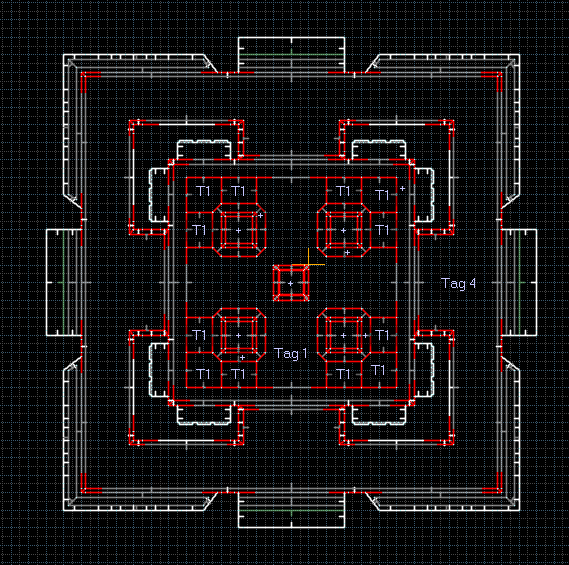
\includegraphics[height=0.6\linewidth]{figures/image.png}
 \end{center}
}

\frameT{Test Maps}{
\begin{center}
	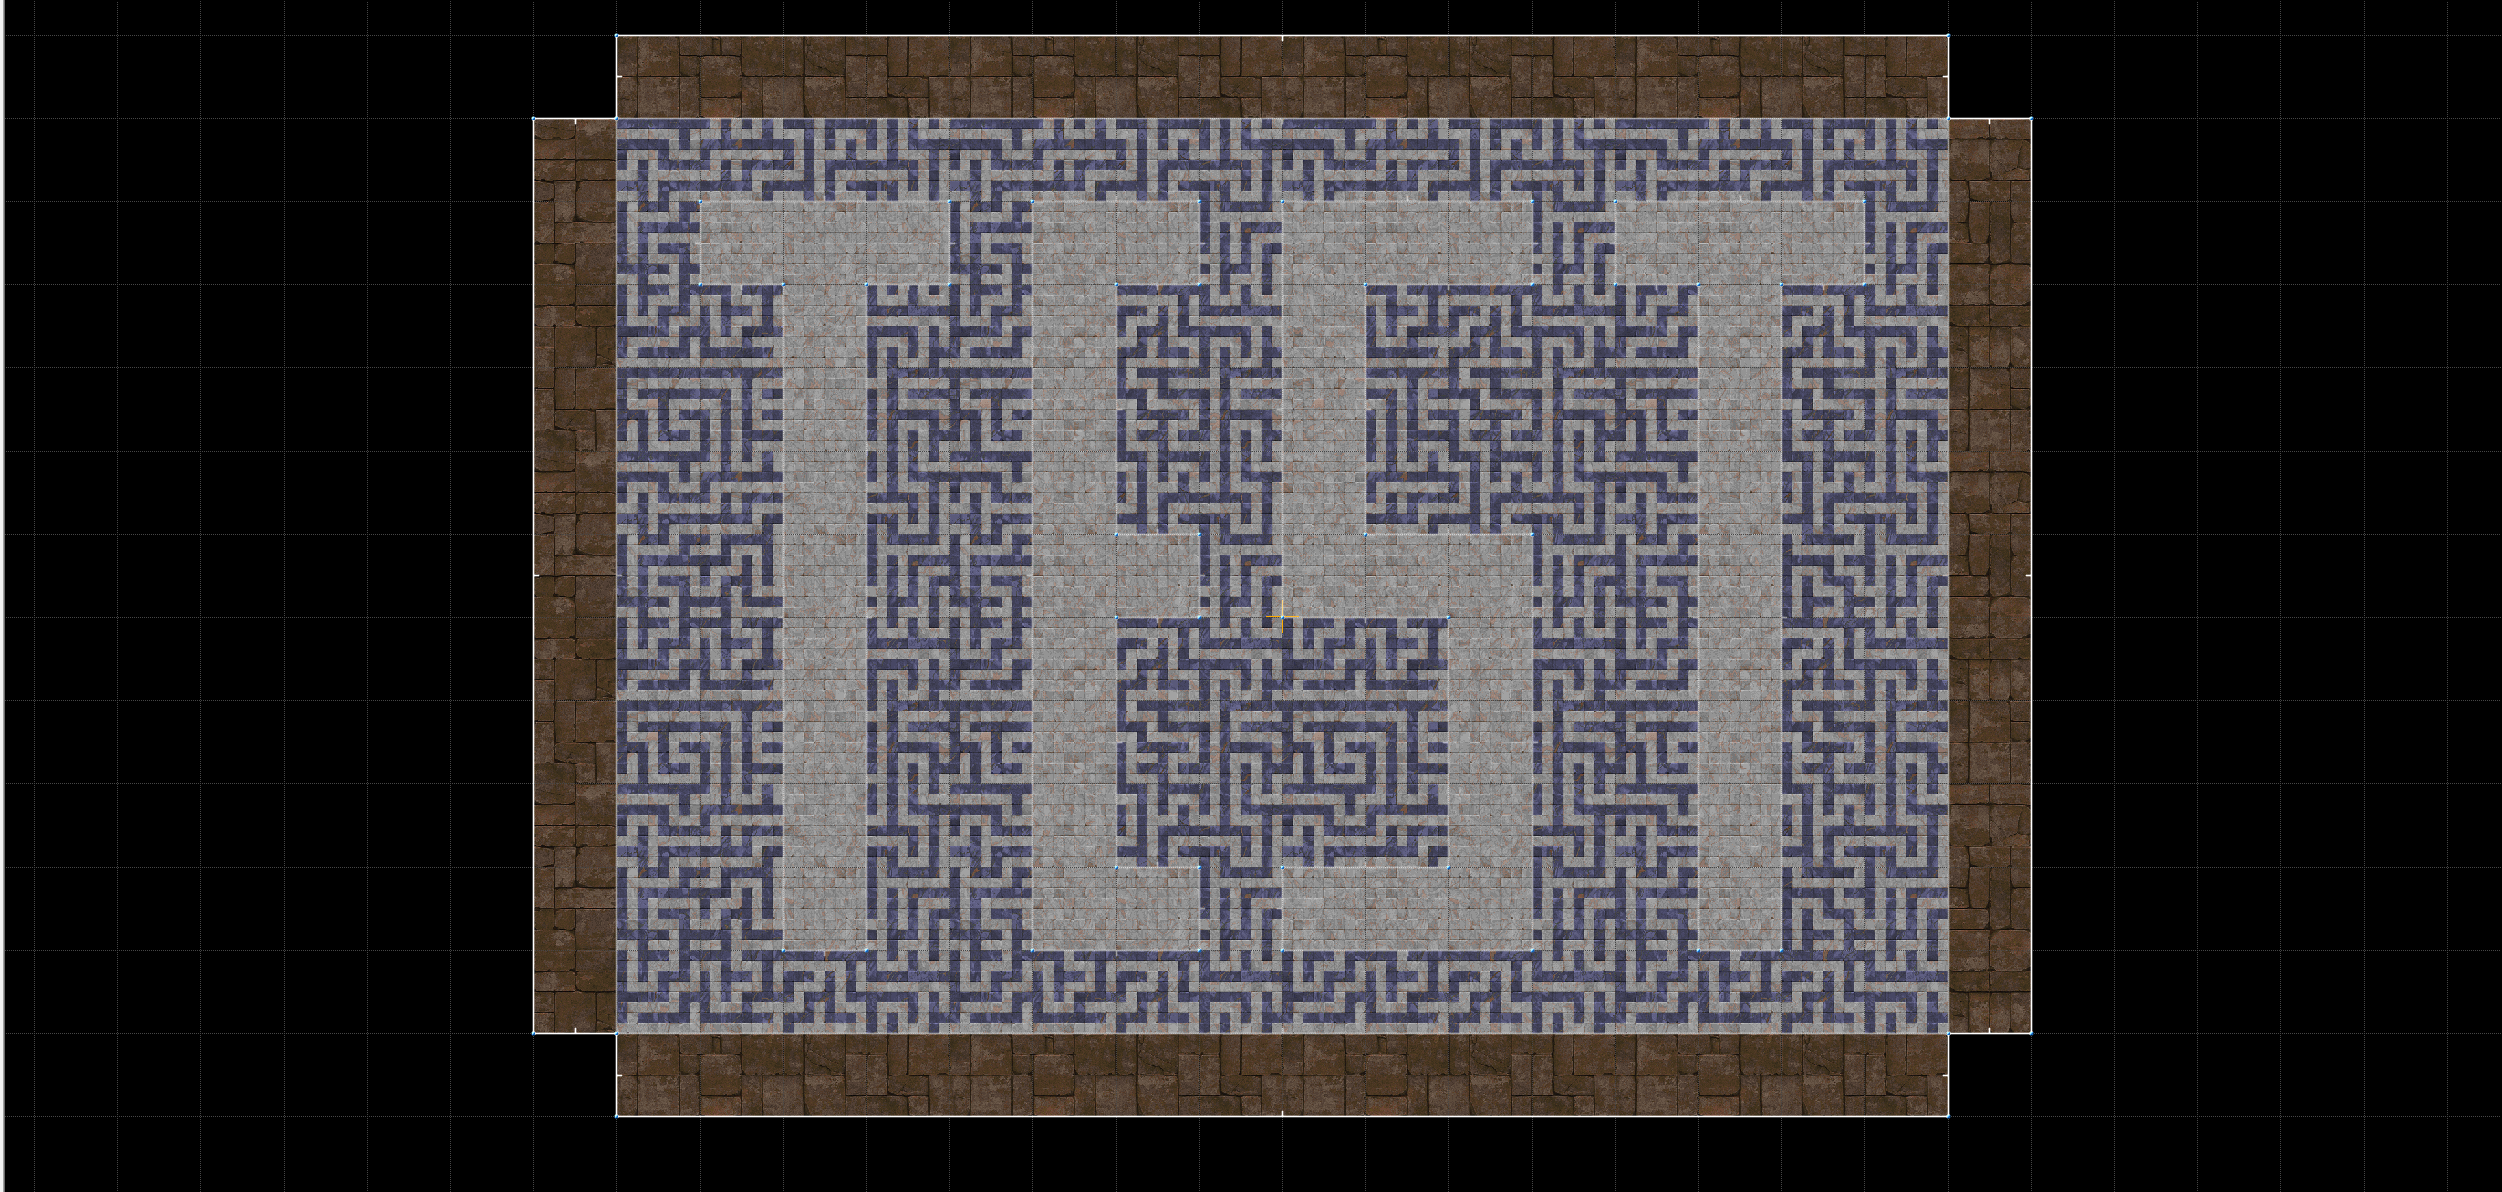
\includegraphics[height=.25\linewidth]{figures/test_map_doom.png}
	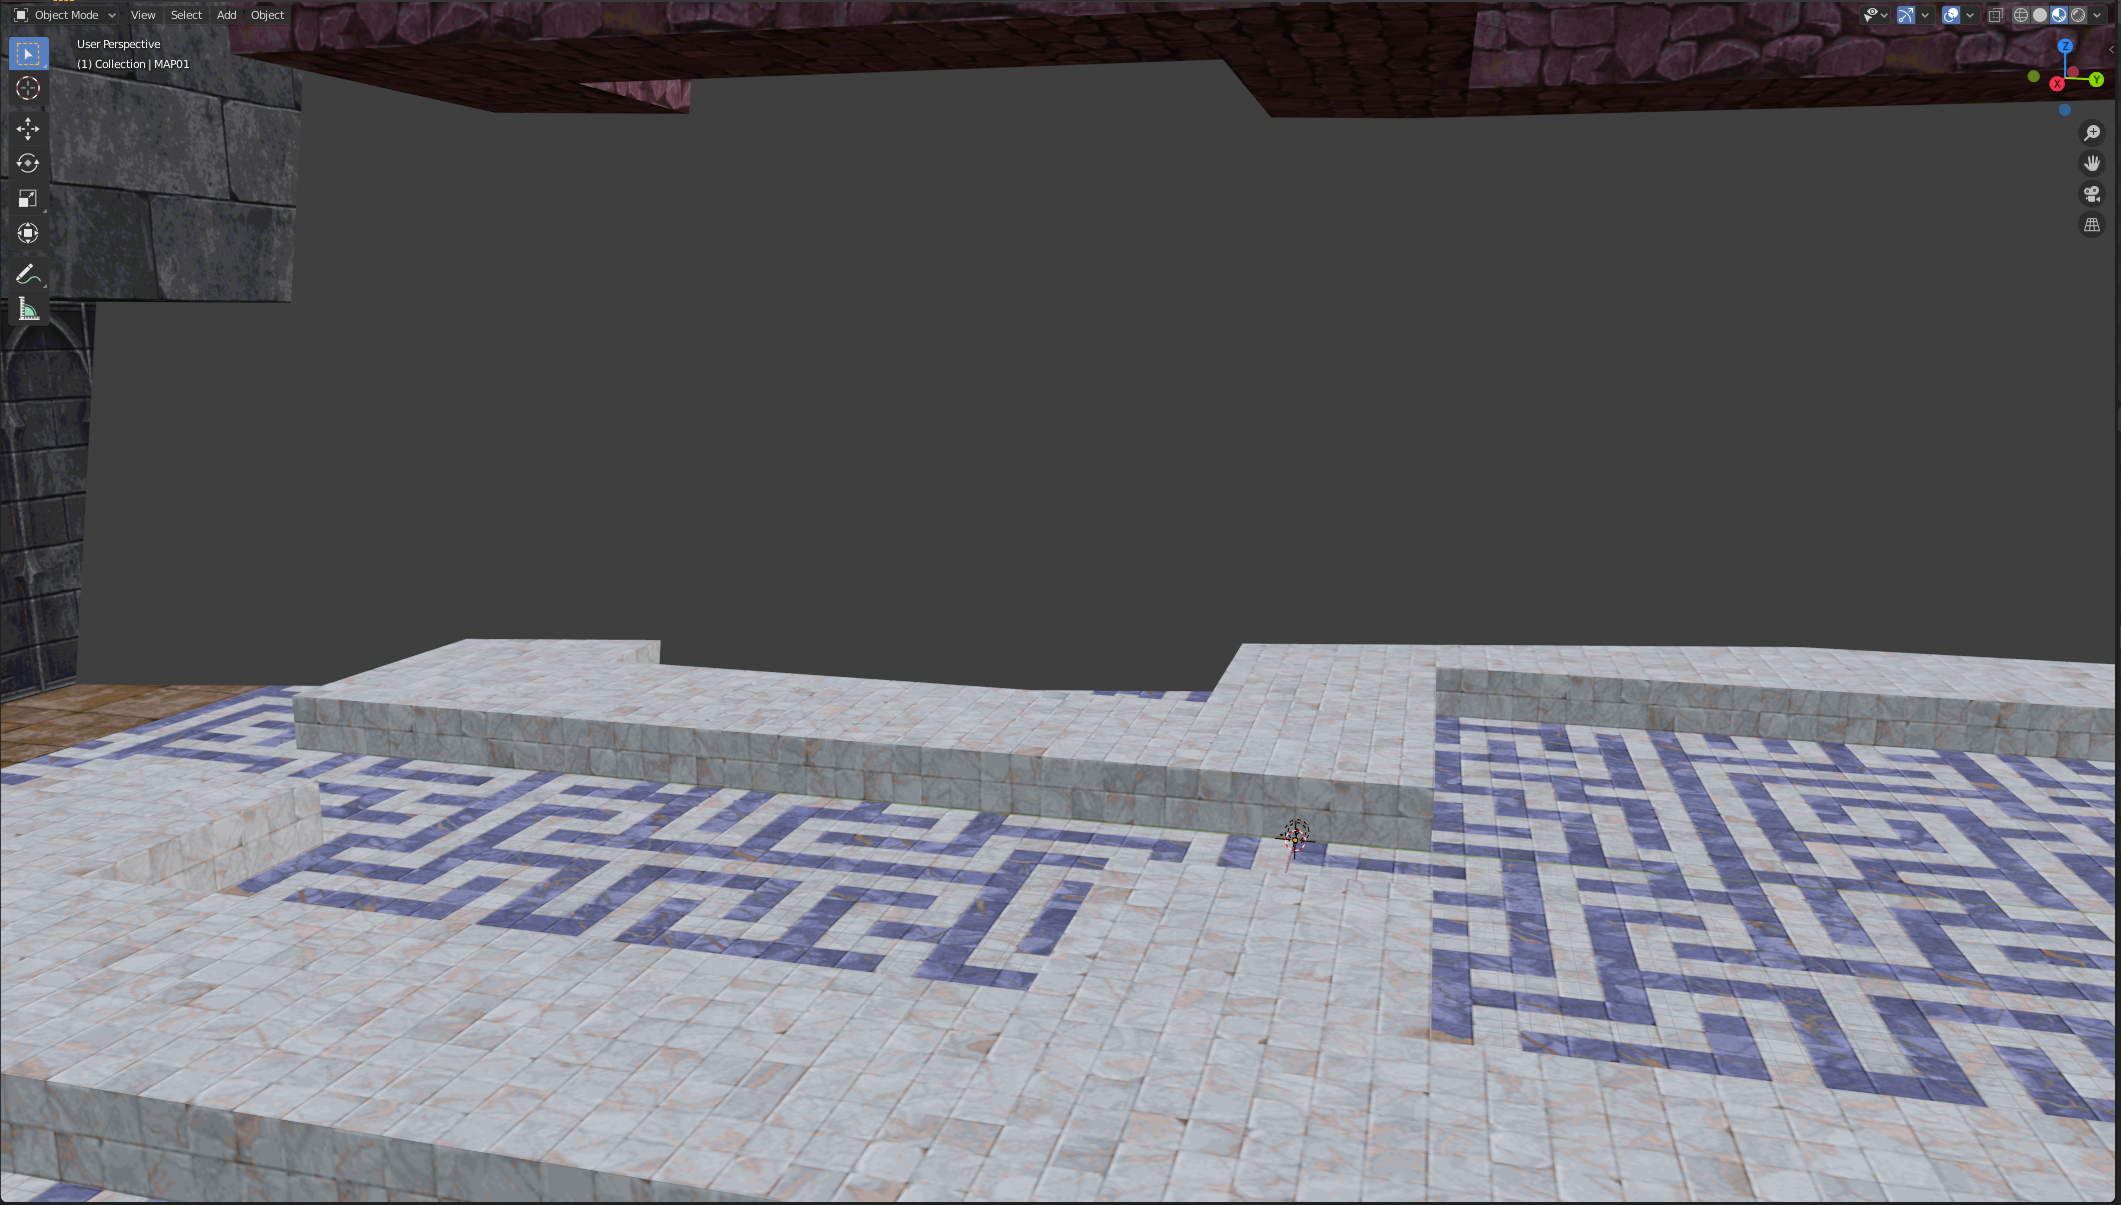
\includegraphics[height=.25\linewidth]{figures/test_map_blender.png}
 \end{center}
 \begin{center}
	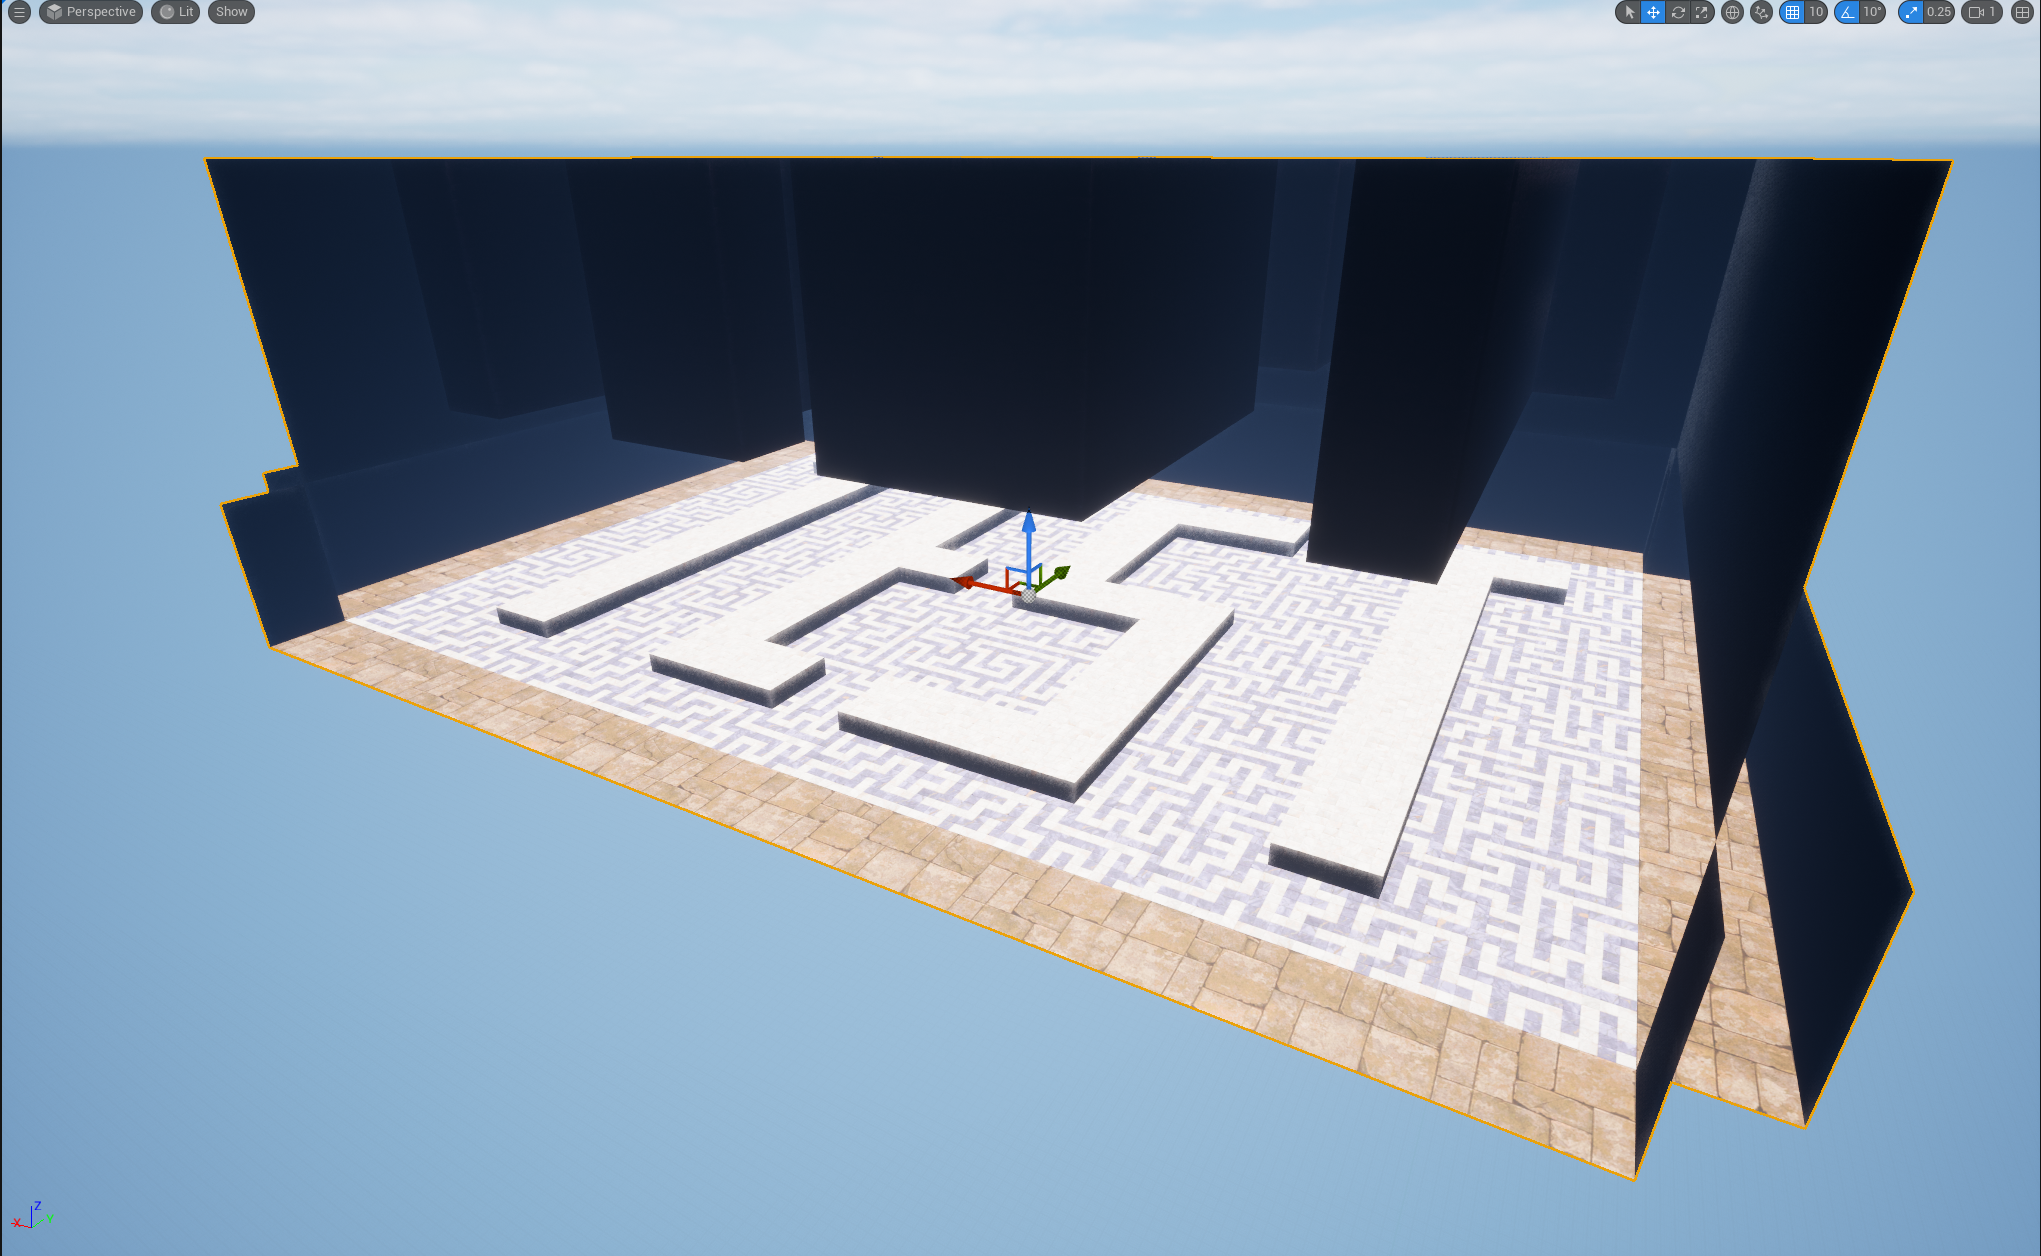
\includegraphics[height=.25\linewidth]{figures/test_map_unreal.png}
 \end{center}
}

\frameT{Map Design} {
  \bigskip
  \begin{itemize}
  	  \item Arena Shooter Map Design
  	  \begin{itemize}
  	  	\item Original multiplayer maps were converted from singleplayer
  	  	\item Modders made maps designed exclusively for multiplayer
  	  	\item Developers followed suit, exclusively multiplayer games emerge
  	  	\bigskip
  	  \end{itemize}
  	  \item Philosophy
      \begin{itemize}
          \item Moving around the map should be smooth
          \item Layout should be easy for the player to quickly learn
          \item Areas of low and high interest
          \bigskip
      \end{itemize}
      \item Layout
      \begin{itemize}
          \item Symmetrical layout to support multiple gamemodes
          \item 'Figure-8' design encourages movement
          \item Multiple areas of interest and connecting areas to encourage fights 
          \bigskip
      \end{itemize}
  \end{itemize}
  \bigskip
}

\section{Effects}
 
\frameT{Effects}{
	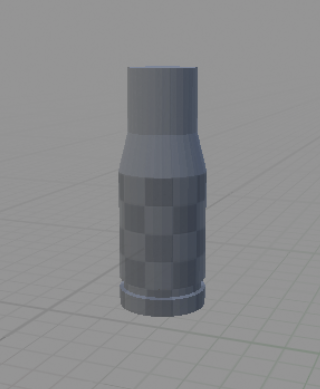
\includegraphics[height=.4\linewidth]{figures/casingModel.png}
 \begin{right}
	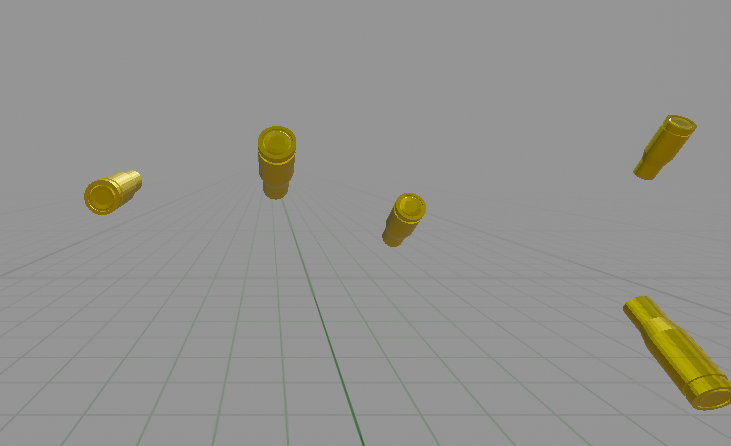
\includegraphics[height=.4\linewidth]{figures/casingEject.png}
 \end{right}
} 

\frameT{Effects}{
 \begin{top}
	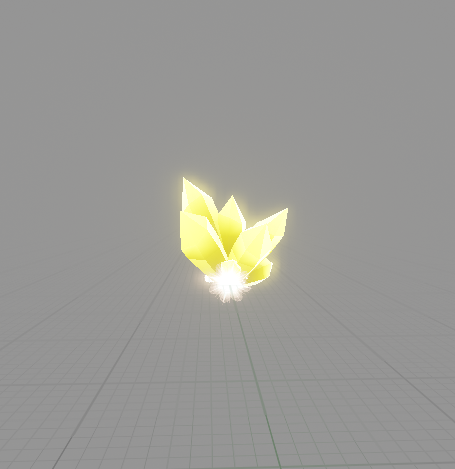
\includegraphics[height=.18\linewidth]{figures/crystal1.png}
        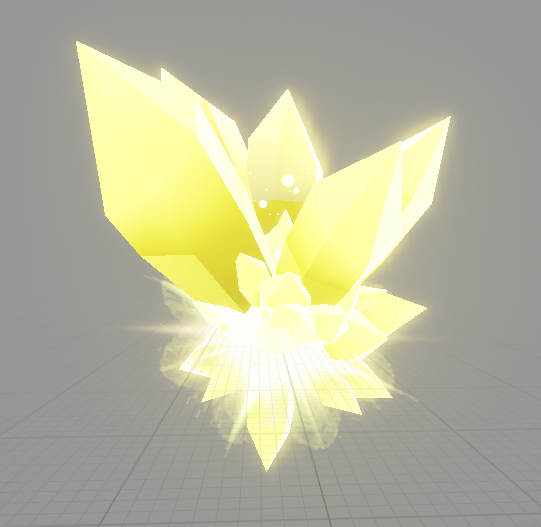
\includegraphics[height=.18\linewidth]{figures/crystal3.png}
        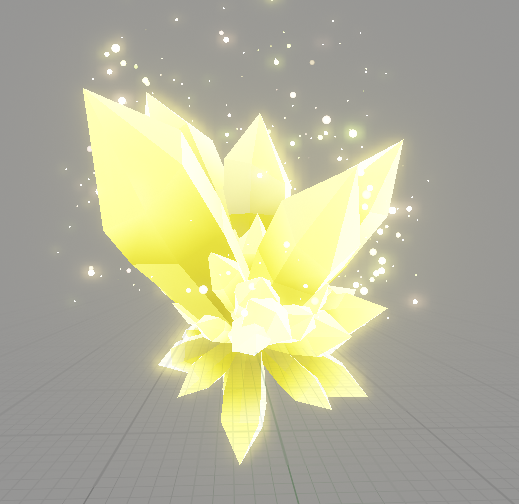
\includegraphics[height=.18\linewidth]{figures/crystal5.png}
        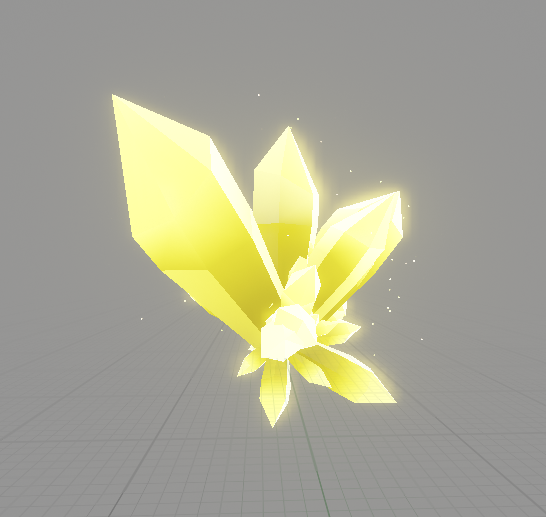
\includegraphics[height=.18\linewidth]{figures/crystal6.png}
        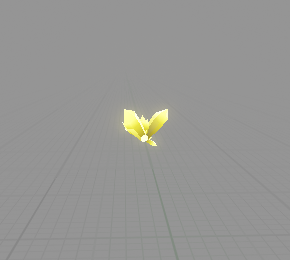
\includegraphics[height=.18\linewidth]{figures/crystal7.png}
 \end{top}
\begin{top}
	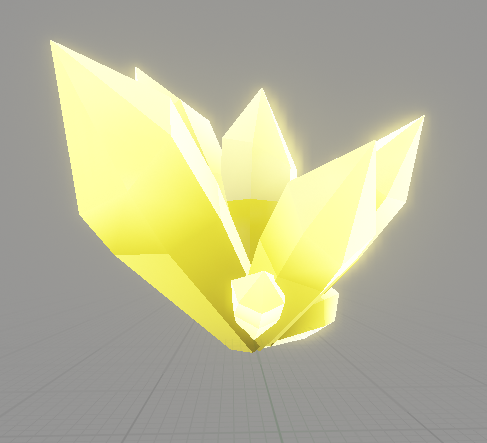
\includegraphics[height=.17\linewidth]{figures/crystalSolo.PNG}
        \includegraphics[height=.17\linewidth]{figures/crystal2Solo.png}
        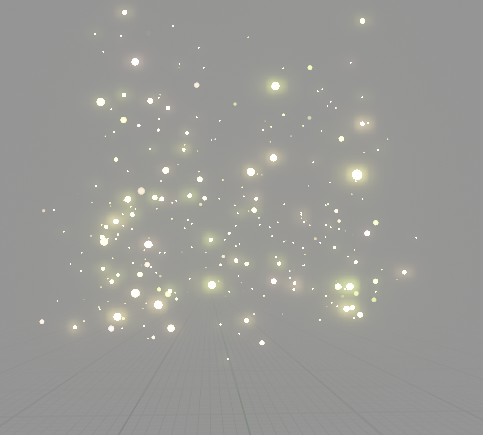
\includegraphics[height=.17\linewidth]{figures/GlitterSolo.PNG}
        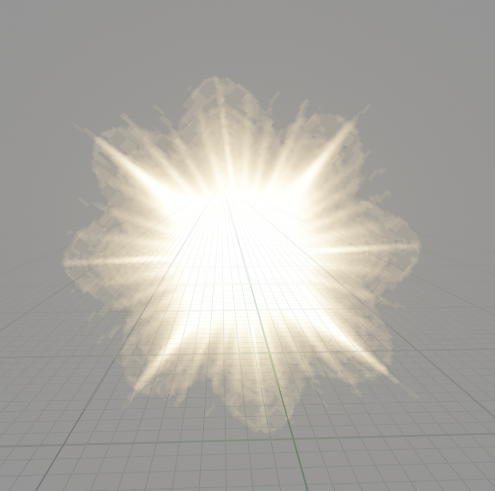
\includegraphics[height=.17\linewidth]{figures/FlashSolo.PNG}
        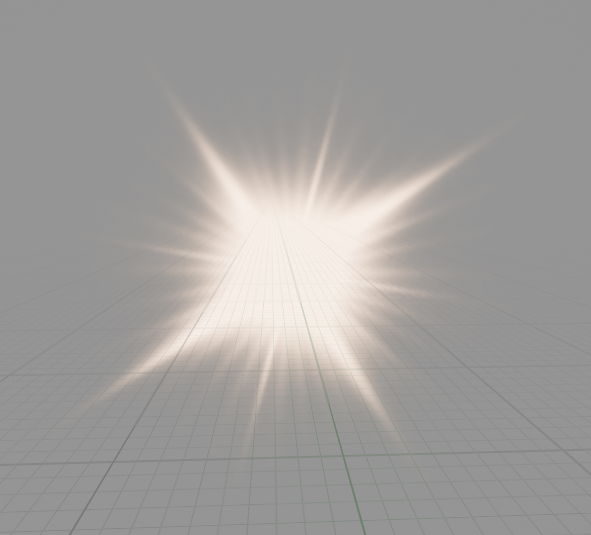
\includegraphics[height=.17\linewidth]{figures/Flash2Solo.PNG}
\end{top}
} 

\section{Modeling}

\frameT{Character Model}{
\begin{center}
	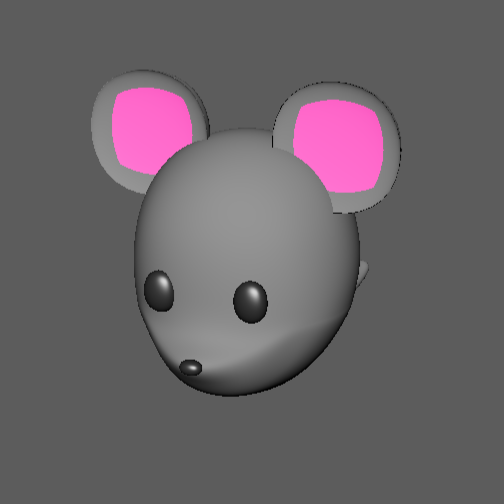
\includegraphics[height=.25\linewidth]{figures/MouseModel.png}
	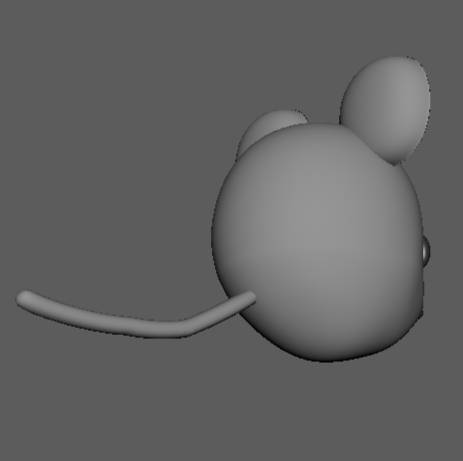
\includegraphics[height=.25\linewidth]{figures/MouseModelBack.png}
 \end{center}
 \begin{center}
 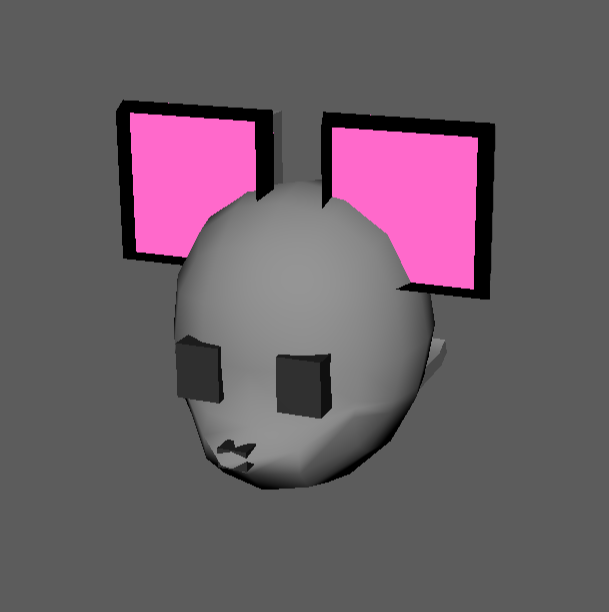
\includegraphics[height=.25\linewidth]{figures/MouseModelUnsmoothed.png}
 \end{center}
} 

\section{Networking}

\frameT{Networking}{
\begin{center}
	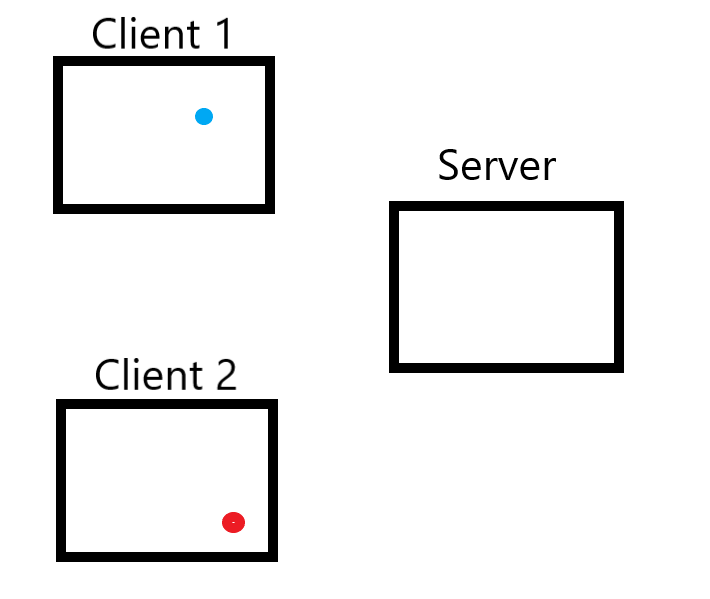
\includegraphics[height=.25\linewidth]{figures/Net1.png}
	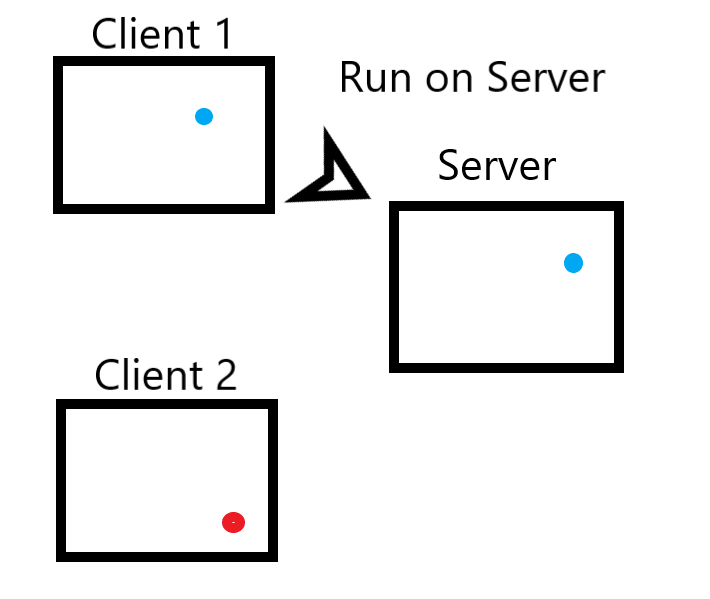
\includegraphics[height=.25\linewidth]{figures/Net2.png}
 \end{center}
 \begin{center}
	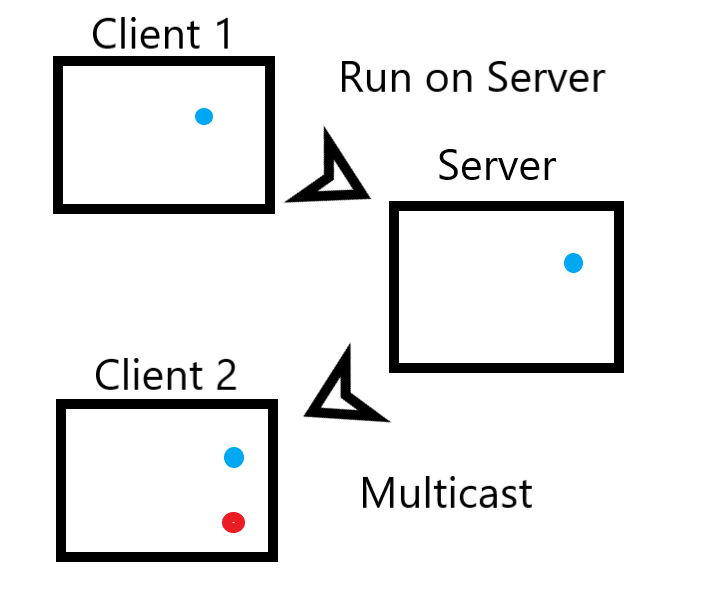
\includegraphics[height=.25\linewidth]{figures/Net3.png}
 \end{center}
}

\frameT{Networking}{
\begin{center}
	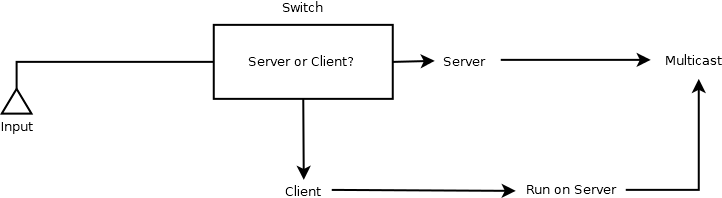
\includegraphics[height=.25\linewidth]{figures/Diagram1.png}
 \end{center}
}

\section{Demo}

\frameT{Demo}{
%Demo of the player in the game environment.
  \begin{figure}[htbp]
  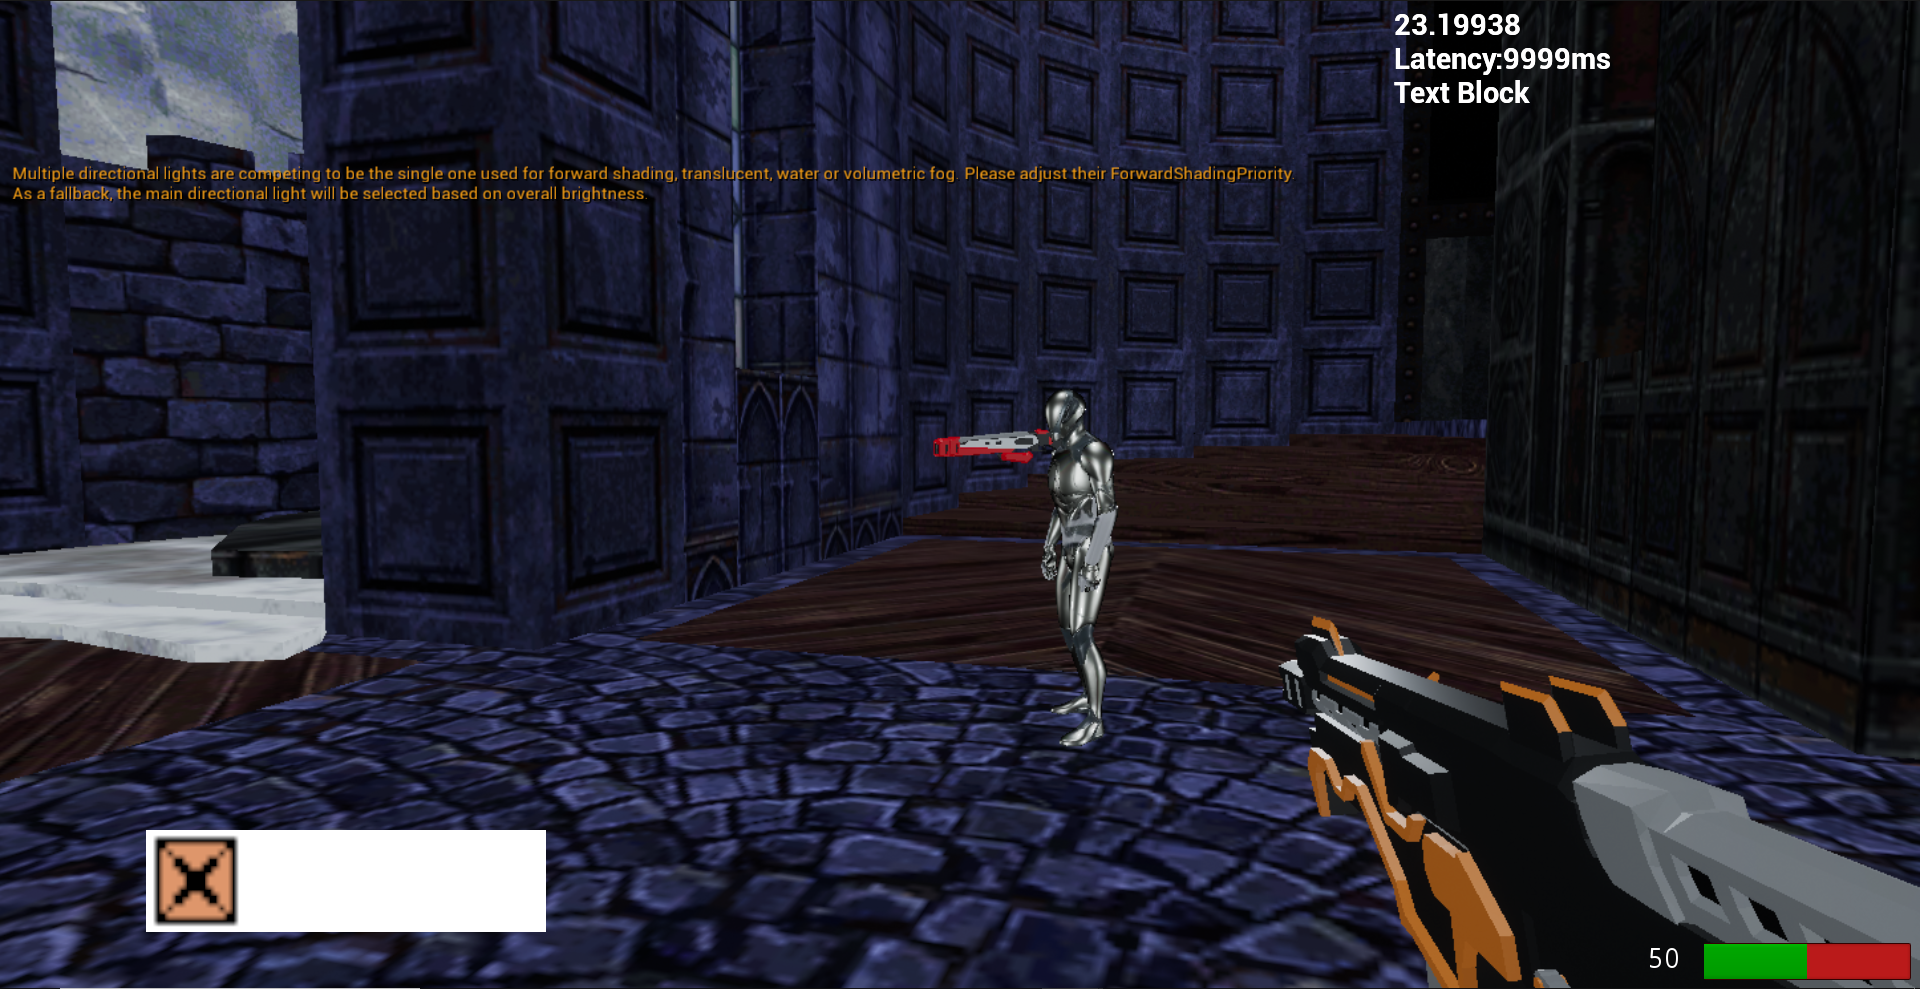
\includegraphics[width=\linewidth,right]{figures/NewTest.png}
  \end{figure}
}

\section{Difficulties}

\frameT{Difficulties}{
  \bigskip
  \begin{itemize}
      \item Networking
      \bigskip
      \item Various weapon related bugs
      \bigskip
      \item Map lighting
  \end{itemize}
}

\section{Conclusion}

\frameT{Future Goals}{
  \bigskip
  \begin{itemize}
      \item Player scores and win conditions
      \bigskip
      \item General clean up of debugging and quality of life improvements.
      \bigskip
      \item More content (maps, weapons, gamemodes, etc.)
  \end{itemize}
}
%\Test Online Video!!!!
%\frameT{Demo}{
%\  Demo of the player in the game environment.
  
%\  \bigskip
  
%\  \href{https://www.youtube.com/watch?v=B03EBcuClKs&ab_channel=JaxxonWoods}{Incase of Emergencies}
%\}








%\begin{frame}[fragile]
%\frametitle{Family Tree Knowledge Base}
%Facts:
%\begin{verbatim}
%Verbatim is a great way of enumerating code/algorithmic ideas.
%\end{verbatim}
%\end{frame}
%
%
%\frameT{How to include images} {
%  %% 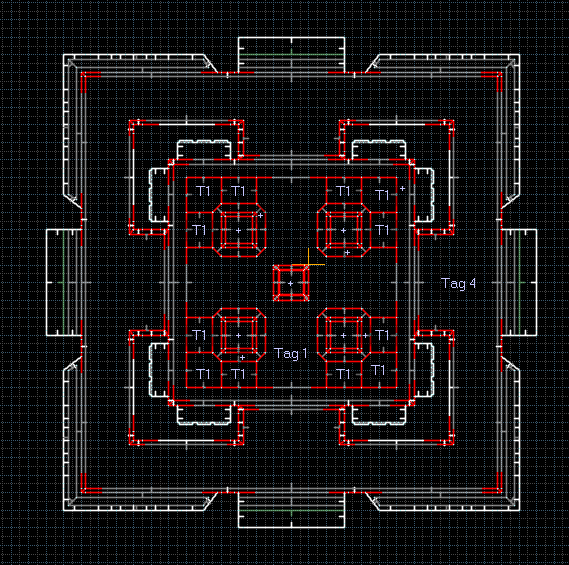
\includegraphics[width=.7\linewidth]{figures/image.pdf}
%}
%
%
%\begin{frame}[fragile]
%  \frametitle{Social Network Graph}
%  \begin{figure}[ht]
%    \begin{minipage}[b]{0.53\linewidth}
%      \centering
%      Minipages are a great way to
%    \end{minipage}
%    \hspace{0.5cm}
%    \begin{minipage}[b]{0.4\linewidth}
%      \centering
%      Line up side-by-side content.
%
%    \end{minipage}
%  \end{figure}
%  
%\end{frame}
%
%
%\frameT{Results} {
%  Describe any results of your work here.
%
%  \bigskip
%
%  Things that worked?
%
%  \bigskip
%
%  Things that didn't work?
%}
%
%\frameT{Conclusions} {
%  Some bullet points here to wrap things up.
%}

\frameT{Any Questions?} {

  \bigskip

  Contact Info:
\begin{enumerate}
    \item Victor Gasior: vicagasi@ut.utm.edu
    \item Blade Johnson: davbjohn@ut.utm.edu
    \item Andrew Newbill: andjnewb@ut.utm.edu
    \item Lucky Woods: lucjwood@ut.utm.edu
\end{enumerate}
\begin{center}
    
\includegraphics[width=.3\linewidth,right]{figures/FA23 Senior Seminar.png}
\end{center}

}

%\frameF{fragile test} {
%}

%% \frameF{Prolog Family Tree} {
%% \begin{verbatim}
%% hello
%% \end{verbatim}



%% }

%Empty Page
%\frameT{Frame 1}{
%}  


\end{document}